%!TEX root = main.tex

%FIRRTL represents the standardized elaborated circuit that the Chisel HDL produces. 
%FIRRTL represents the circuit immediately after Chisel's elaboration but before any circuit simplification. It is designed to resemble the Chisel HDL after all meta-programming has executed. Thus, a user program that makes little use of meta-programming facilities should look almost identical to the generated FIRRTL.

%For this reason, 

\zhilin{Can we find a running example ?}

Below is an example of FIRRTL programs.
\begin{lstlisting}
circuit MyCircuit:
  module MyModule :
    input in: UInt[3]
    input n: UInt<2>
    output out: {valid: UInt<1>, ready: UInt<1>,  result: UInt<1>}
    when eq(n, UInt(0)) :
      out.valid <= in[0]
    else when eq(n, UInt(1)) :
      out.ready <= in[1]
    else when eq(n, UInt(2)) :
      out.result <= in[2]
\end{lstlisting}
A FIRRTL \emph{circuit} comprises modules, each of which include several ports and statements. 
Each \emph{port} has an identifier and types and is either an input or output. 
A \emph{module} includes ports and  a sequence of statements. 
%A \emph{port}  is either an input port or an output port, and has an identifier as well as a type. 
Each \emph{statement} defines a wire, register, node, connect (<=) or partial connect (<-), or conditional (when), and so on. 
%A \emph{statement} is either a declaration of wire, register, instance, node, or a connection (<=) or partial connection (<-), or a conditional (when) statement. 
A \emph{type} can be either a \emph{ground type}, e.g. \begin{lstinline}!UInt<2>!\end{lstinline} (unsigned integer of bit width 2), or an \emph{aggregate type}, which is either a \emph{vector type}, e.g. \begin{lstinline}!UInt[3]!\end{lstinline} (a three element vector of unsigned integers), or a \emph{bundle type} e.g \begin{lstinline}! {valid: UInt<1>, ready: UInt<1>,  result: UInt<1>} !\end{lstinline} which comprises three signals of the ground type  \begin{lstinline}!UInt<1>!\end{lstinline}. 
The syntactic rules of FIRRTL are given in Figure~\ref{fig-firrtl-synt-simp}. Note that these rules are in Extended Backus–Naur form, where {· · · } denotes repetition (possibly empty) and [· · · ] denotes option, moreover, the terminals are doubly quoted. Moreover,  the syntactic rules of FIRRTL presented here is a simplification of those in the official specification\footnote{\url{https://github.com/chipsalliance/firrtl-spec/blob/main/spec.md}}. For instance, indent, dedent and newline terminals are omitted for readability, moreover, the type and constructions for analog signals are also omitted, since we focus on digital circuits in this work.

%\begin{itemize}
%\item A circuit in FIRRTL consists of modules, each of which include several ports and statements. 
%\item Each port has an identifier and types and is either an input or output. 
%\item Each statement defines a wire, register, memory, or node, connect (<=) or partial connect (<-), attach (for analog signals), or conditional (when), and so on.  
%\item Expressions are widely used in statements. Each expression is an unsigned/signed integer constant, a reference, a multiplexer, a validif expression, or an expression obtained by applying primitive operations on ground types. 
%\item A ground type is ``Clock'', ``Reset'', ``AsyncReset'', ``UInt'' (unsigned integer), ``SInt'' (signed integer), ``Analog'', or ``Fixed'' (fixed point number).  
%\item An aggregate type is either declared by describing the (possibly nested) fields, or an array (e.g. UInt[10]).
%\end{itemize}



\begin{figure}[htbp]
{\footnotesize
\[
\begin{array}{l l l}
%\mbox{\bf Circuit} & 
c & ::= & \mbox{\tt ``circuit''}\ id\mbox{\tt ``:''} \{m\}\\
%
%\mbox{\bf Module} & 
m & ::= & \mbox{\tt ``module''} \ id \{p\} \{s\}\\
%
%\mbox{\bf External Module} & 
%em & ::= & \mbox{\tt ``extmodule''}\ id \{p\} [\mbox{\tt ``defname =''}\ id] \{\mbox{\tt ``parameter''}\ id \mbox{\tt ``= ''}(string \mid int)\}\\
%
%\mbox{\bf Port} & 
p & ::= & (\mbox{\tt ``input''} \mid \mbox{\tt ``output''})\ id\mbox{\tt ``:''}t \\
%
 %\mbox{\bf Statment} & 
 s & ::= & \mbox{\tt ``wire''}\ id\mbox{\tt ``:''}t  \mid \mbox{\tt ``reg''}\ id\mbox{\tt ``:''}t\ e [\mbox{\tt ``(with:\{reset=>(''} e\mbox{\tt ``,''} e \mbox{\tt ``)\})''}] \\
 %& 
  &   &  \mid
%  \mid memory \mid 
  \mbox{\tt ``inst''}\ id\ \mbox{\tt ``of''}\ id \mid \mbox{\tt ``node''}\ id \mbox{\tt ``=''} id  \mid r \mbox{\tt ``<=''} e  \mid r \mbox{\tt ``<-''} e \mid r\ \mbox{\tt ``is invalid''} \\ 
%&  
&   &\mid \mbox{\tt ``when''}\ e\mbox{\tt ``:''}\{s\} [\mbox{\tt ``else:''} \{s\}] \mid \mbox{\tt ``skip''}\\ 
%
%\mbox{\bf Memory} & 
%memory & = &  \mbox{``mem''}, id, newline, indent, \\
 %& 
% & & \mbox{``data-type''}, \mbox{``=>''}, type, newline, \\
 %& 
% & & \mbox{``depth''}, \mbox{``=>''}, int, newline, \\
 %& 
% & & \mbox{``read-latency''}, \mbox{``=>''}, int, newline, \\ 
 %& 
% & & \mbox{``write-latency}, \mbox{``=>''}, int, newline,  \\
 %& 
% & & \mbox{``read-under-write''}, \mbox{``=>''}, ruw, newline, \\
  %& 
%  & & \{\mbox{``reader''}, \mbox{``=>''}, id, newline\}, \\
  %& 
%  & & \{\mbox{``writer''}, \mbox{``=>''}, id, newline\}, \\
  %& 
%  & & \{\mbox{``readwriter''}, \mbox{``=>''}, id, newline\}, dedent;\\    
%
%\mbox{\bf Read Under Write Flag} & 
%ruw & = & \mbox{``old''} \mid \mbox{``new''} \mid \mbox{``undefined''};\\
%
%\mbox{\bf Expression} & 
e & ::= & (\mbox{\tt ``UInt''} | \mbox{\tt ``SInt''}) [w] \mbox{\tt ``(''}int\mbox{\tt ``)''} \mid r \mid \mbox{\tt ``mux(''}e\mbox{\tt ``,''} e\mbox{\tt ``,''} e\mbox{\tt ``)''} \mid \mbox{\tt ``read(''}sr \mbox{\tt ``)''} \mid op\\
%
%& 
r & ::= & sr \mid r \mbox{\tt ``[''} e \mbox{\tt ``]''}\\
%
sr & ::= & id \mid sr\mbox{\tt ``.''}id \mid sr\mbox{\tt ``[''}int\mbox{\tt ``]''}\\
%& 
w & ::= & \mbox{\tt ``<''} int \mbox{\tt ``>''}\\
%
%& 
%binarypoint & = & \mbox{``<''}, \mbox{``<''}, int, \mbox{``>''}, \mbox{``>''};\\
%
 %\mbox{\bf Bundle Field} & 
%
%\mbox{\bf Data Types} & 
t & ::= & tg \mid ta \\
 %& 
 tg & ::= &  \mbox{\tt ``Clock''} \mid \mbox{\tt ``Reset''} \mid \mbox{\tt ``AsyncReset''} \mid (\mbox{\tt ``UInt''} \mid \mbox{\tt ``SInt''}) [w] \\
 %& 
% & & \mid \mbox{``Fixed''}, [width], [binarypoint];\\
 %& 
%
  ta & ::= &\mbox{\tt ``\{''} f \{f\}\mbox{\tt ``\}''} \mid t \mbox{``[''} int \mbox{``]''} \\
%
    f & ::= & [\mbox{\tt ``flip''}]\ id\mbox{\tt ``:''}t\\
%& & & \mbox{``UInt''}, [\mbox{``<''}, int, \mbox{``>''}] \mid \mbox{``SInt''}, [\mbox{``<''}, int, \mbox{``>''} ] \\
%& & & \mid \mbox{``Fixed''}, [\mbox{``<''}, int, \mbox{``>''} ] [\mbox{``<}\mbox{<''}, int, \mbox{``>}\mbox{>''}]\\
% &  &  & \mid \mbox{``Clock''} \mid \mbox{``Analog''},  [\mbox{``<''}, int, \mbox{``>''}] \mid \mbox{``\{''}, field, \mbox{``\}''} \mid type, \mbox{``[''}, int, \mbox{``]''}; \\
%
id & ::= & ( \mbox{\tt ``\_''} \mid l) \{ \mbox{\tt ``\_''} \mid l \mid d\} \\
%\mbox{\bf Primitive Operation} & 
op & ::= & op\_2e \mid op\_1e \mid op\_1e1i \mid op\_1e2i \\
%& 
op\_2e & ::= & op\_2e\_key \mbox{\tt ``(''}  e \mbox{\tt ``,''}  e \mbox{\tt ``)''} \\
%
%& 
op\_2e\_key & ::= &  \mbox{\tt ``add''}  \mid  \mbox{\tt ``sub''}  \mid \mbox{\tt ``mul''} \mid \mbox{\tt ``div''} \mid \mbox{\tt ``mod''} \mid \mbox{\tt ``lt''} \mid \mbox{\tt ``leq''} \mid \mbox{\tt ``gt''} \mid \mbox{\tt ``geq''} \mid \mbox{\tt ``eq''} \mid \mbox{\tt ``neq''} \\
%& 
& &   \mid \mbox{\tt ``dshl''}  \mid \mbox{\tt ``dshr''} \mid \mbox{\tt ``and''} \mid \mbox{\tt ``or''} \mid \mbox{\tt ``xor''} \mid \mbox{\tt ``cat''} \\
 %
%& 
op\_1e & ::= & op\_1e\_key \mbox{\tt ``(''}  e \mbox{\tt ``)''} \\
%& 
op\_1e\_key & ::= & \mbox{\tt ``asUInt''} \mid \mbox{\tt ``asSInt''} \mid \mbox{\tt ``asClock''} \mid \mbox{\tt ``cvt''} \mid \mbox{\tt ``neg''} \mid \mbox{\tt ``not''}  \mid \mbox{\tt ``andr''} \mid \mbox{\tt ``orr''} \mid  \mbox{\tt ``xorr''}\\
%
%& 
op\_1e1i & ::= & op\_1e1i\_key \mbox{\tt ``(''}  e \mbox{\tt ``,''} int \mbox{\tt ``)''} \\
%& 
op\_1e1i\_key & ::= & \mbox{\tt ``pad''} \mid \mbox{\tt ``shl''} \mid \mbox{\tt ``shr''} \mid \mbox{\tt ``head''} \mid \mbox{\tt ``tail''} \\
%& 
op\_1e2i & ::= & op\_1e2i\_key \mbox{\tt ``(''}  e \mbox{\tt ``,''}  int  \mbox{\tt ``,''}  int \mbox{\tt ``)''} \\
%& 
op\_1e2i\_key & ::= & \mbox{\tt ``bits''}\\
%
int & ::= & [\mbox{\tt ``-''}] d \{d\} \mid \mbox{\tt ``"b''} [\mbox{\tt ``-''}] d\_b \{d\_b\} \mbox{\tt ``"''} 
 \mid \mbox{\tt ``"o''} [\mbox{\tt ``-''}] d\_o \{d\_o\} \mbox{\tt ``"''} \mid 
\mbox{\tt ``"h''} [\mbox{\tt ``-''}] d\_h \{d\_h\} \mbox{\tt ``"''}
%
%\mbox{\bf File Information Token} & 
%info & = & \mbox{``@''}, \mbox{``[''}, \{string, \mbox{`` ''}, linecol\}, \mbox{``]''};\\
%& 
%linecol & = &  digit\_dec, \{digit\_dec\}, \mbox{``:''}, digit\_dec, \{digit\_dec\};\\
%& 
%
\end{array}
\]
}
\caption{Syntax of FIRRTL}
\label{fig-firrtl-synt-simp}
\end{figure}

From the syntax, FIRRTL features the high-level constructs like vector types, bundle types, conditional statements, connects, partial connects, and modules.
These high-level constructs are then gradually removed by a sequence of lowering transformations. During each lowering transformation, the circuit is rewritten into an equivalent circuit using simpler, lower-level
constructs. Eventually the circuit is simplified to its most restricted form, resembling a structured netlist, which allows for easy translation to an output language (e.g. Verilog). This form is given the name lowered FIRRTL (LoFIRRTL) and is a strict subset of the full FIRRTL language. For clarity, the original form is called high FIRRTL (HiFIRRTL). 

\zhilin{stopped here}

A FIRRTL circuit is defined to be a valid LoFIRRTL circuit if it obeys the following restrictions:
\begin{itemize}
\item All widths must be explicitly defined.
\item The conditional statement is not used.
\item All components are connected to at most once.
\item All components must be declared with a ground type.
\item The partial connect statement is not used.
\end{itemize}
Intuitively, LoFIRRTL is in a flavor similar to static single-assignment (SSA) form of software programs. Programs in SSA form are those where each variable is assigned exactly once, and each variable is defined before it is used.

Besides LoFIRRTL, there is another lowered form of FIRRTL, MidFIRRTL. Nevertheless, in this paper, we ignore MidFIRRTL, since there are no requirements in FIRRTL related to accepting or producing MidFIRRTL.

\begin{figure}[htbp]
\centering
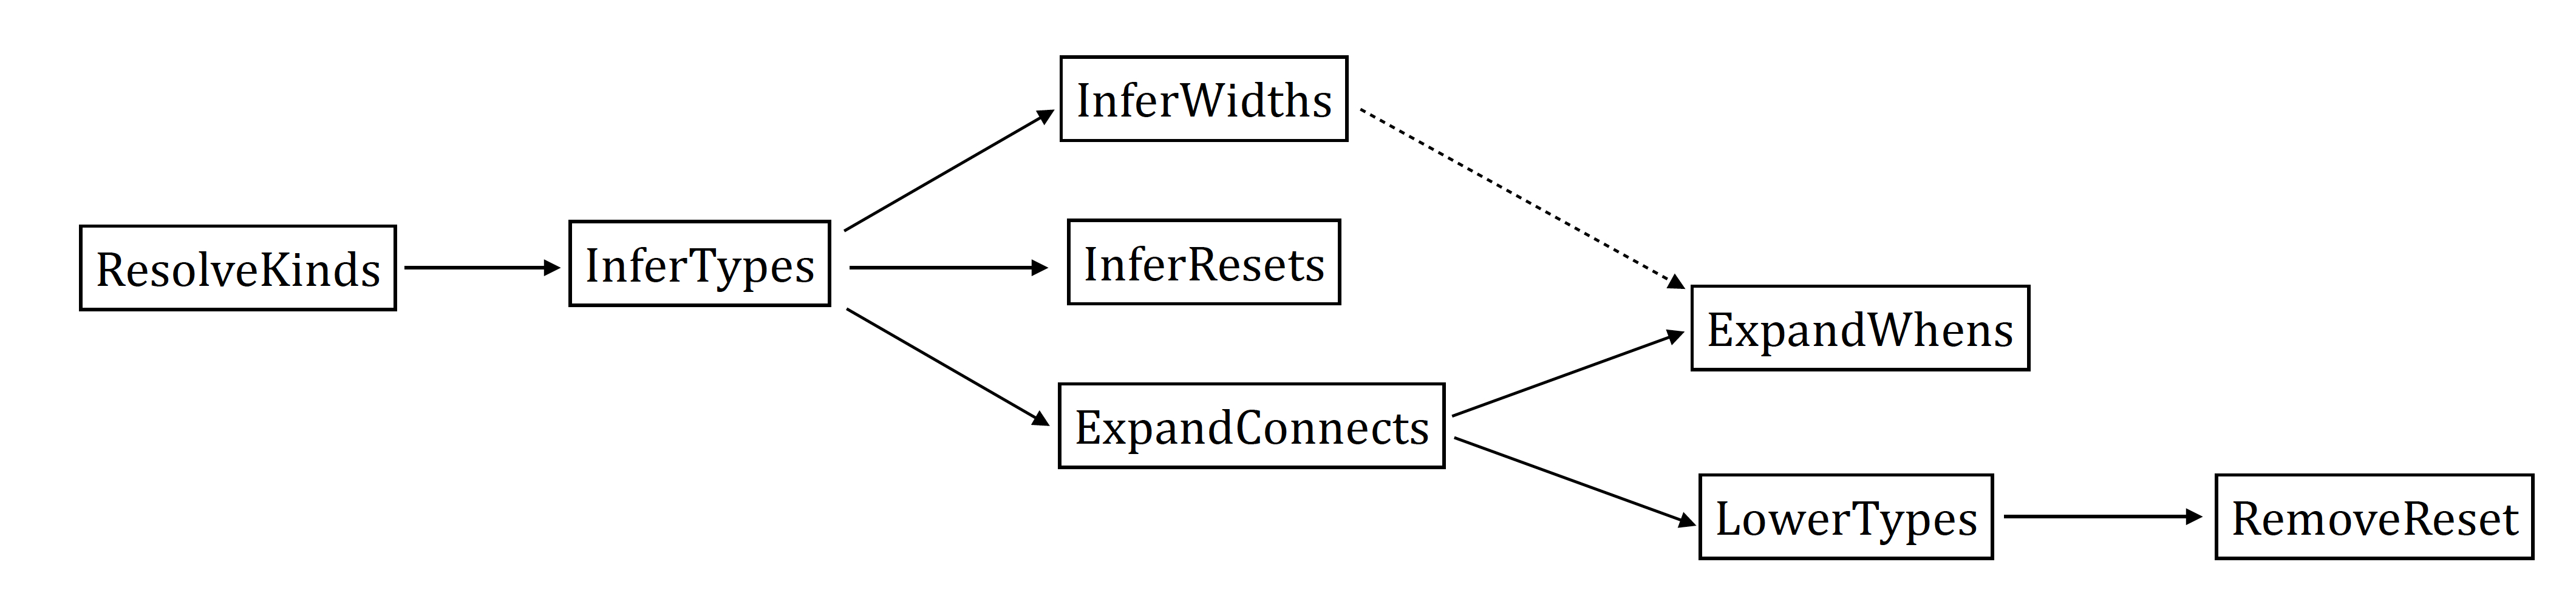
\includegraphics[width = 0.8\textwidth]{firrtl-compilation-passes.jpg}
\caption{Dependencies between FIRRTL compilation passes}
\label{fig-c-pass}
\end{figure}

HiFIRRTL programs are compiled into LoFIRRTL programs by the following compilation passes,
\begin{itemize}
%\item ResolveKinds that resolves the k
%
\item InferTypes that infer the types of components, e.g. wires, nodes, registers,
%
\item InferWidths that infer the bit-width of ground types,
%
\item InferResets that infers concrete resets, i.e. AsyncReset or UInt<1>,
%
\item ExpandConnects that expands the connect statements, 
%
\item ExpandWhens that expands the when statements, 
%
\item LowerTypes that lower down the aggregate types, i.e. bundle and vector types, 
%
\item RemoveReset that removes synchronous resets. 
\end{itemize}
The dependencies between these compilation passes are illustrated in Figure~\ref{fig-c-pass}.

